\subsection{Chorregentendienst mit Unterbrechung}

\hypertarget{RefHeadingToc100333732}{}Zum 1. September 1921 wurde, dem
Protokoll der Kirchenverwaltungssitzung zufolge, August Högn der
Chorregenten- und Organistendienst provisorisch übertragen.\footnote{
Dokument Nr. 116, Protokoll der Kirchenverwaltungssitzung, 21.8.1921}
Provisorisch steht hier nur deshalb, weil ein Jahr zuvor die gesetzlich
geregelte Verbindung zwischen Schul- und Kirchendienst, die mittels der
Chorregenten-, Organisten- und Mesnertätigkeiten der Lehrer bestand,
abgeschafft worden war. Besonders am Vormittag stattfindende
Beerdigungen standen der längerfristigen Weiterführung des
Organistendienst durch die Lehrer im Weg. Da viele Lehrer sich
freiwillig bereit erklärten, weiterhin Chorregent zu bleiben, ließ sich
diese jahrhunderte alte Tradition nicht von heute auf morgen
abschaffen. Den Schulbehörden blieb anscheinend nichts anderes übrig,
als den Chorregentendienst der Lehrer, verbunden mit den
Stundenausfällen, zumindest für eine gewisse Übergangszeit zu dulden.

\begin{center}
\begin{minipage}{9.491cm}
\begin{flushleft}
\tablefirsthead{}
\tablehead{}
\tabletail{}
\tablelasttail{}
\begin{supertabular}{m{4.8960004cm}m{4.196cm}}

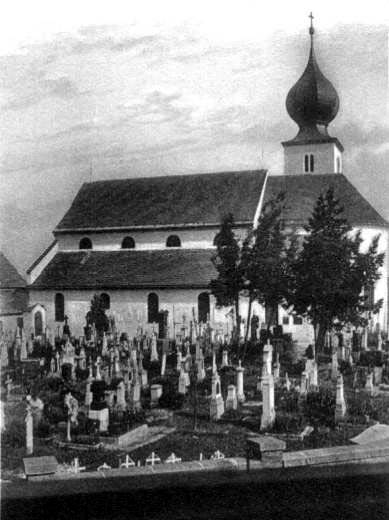
\includegraphics[width=4.713cm,height=6.301cm]{pictures/zulassungsarbeit-img025.jpg}

Abb. \stepcounter{Abb}{\theAbb}: Pfarrkirche St. Laurentius zur Zeit von
August Högn &

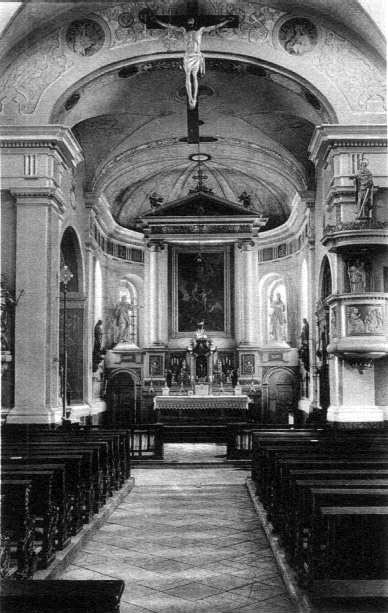
\includegraphics[width=4.013cm,height=6.292cm]{pictures/zulassungsarbeit-img026.jpg}

Abb. \stepcounter{Abb}{\theAbb}: Blick zum Altarraum\\
\end{supertabular}
\end{flushleft}
\end{minipage}
\end{center}
Eine weitere Tradition, nämlich dass der Schulleiter den
Chorregentendienst übernahm, \footnote{Dokument Nr. 55, Artikel in der
Reicheneder-Chronik über August Högn} wurde in Ruhmannsfelden
fortgeführt, obwohl der Kirchendienst der Lehrer offiziell abgeschafft
wurde, als August Högn nach der Pensionierung des Bezirkshauptlehrers
Alois Auer 1921 \footnote{Reicheneder-Chronik, Pfarrmesner, Blatt 1
Vorderseite} nicht nur Chorregent, sondern
auch Schulleiter wurde. Max Weig war von 1879 bis zu seinem Tod 1895
Schulleiter und somit auch Organist und Chorregent.\footnote{
Reicheneder-Chronik, Schulwesen, Blatt 100
Rückseite}Erst im seinem Todesjahr kam vom
königlichen Bezirksamt Viechtach die Anweisung, dass ein Hilfslehrer
den Chorregentendienst übernehmen sollte. \footnote{Dokument Nr. 1,
Brief von Bezirkshauptmann Heerwagen an Kirchenverwaltung, 18.1.1895}
Von 1895 bis 1921 \footnote{Reicheneder-Chronik, Schulwesen, Blatt 110
Vorderseite} leitete Weigs Nachfolger, der Schulleiter Alois Auer,
zusammen mit seiner Frau Anna den Chor, ehe Högn ihn
fortführte. \footnote{Dokument Nr. 6, Brief von Max Rauscher sen. an
Kirchenverwaltung, 14.3.1927}

Vor allem aber dürften seine überdurchschnittlichen musikalischen
Fähigkeiten Högn dazu bestimmt haben, die alte Tradition des Lehrers
und Chorregenten in Personalunion weiterzuführen. Bevor er die
Kirchenchorleitung übernahm, hatte er über 20 lang Jahre als
guter \footnote{Dokument Nr. 48, Zeitungsartikel aus Viechtacher
Bayerwald-Bote, 2.8.1958} Tenor \footnote{Interview Nr. 5, Barbara
Essigmann, 2.1.2003, Absatz 40} und versierter Organist – man sagte von
ihm, dass er gleichzeitig singen, spielen und dirigieren
konnte \footnote{Interview Nr. 16, Maria Freisinger, 25.8.2004, Absatz
28} – in verschiedenen Orten an der Kirchenmusik mitgewirkt und
Erfahrungen gesammelt. \footnote{Dokument Nr. 18, Brief von August Högn
an Pfarrer Reicheneder, 25.1.1954} Nicht nur im Manualspiel war er
gewandt, wie die virtuos gesetzte Fassung seines Marsches „In Treue
fest!“ für Klavier zu zwei Händen beweist, sondern auch mit dem
Pedaleinsatz konnte er von seinem Können überzeugen.\footnote{
Interview Nr. 4, Maria Schröck, 30.12.2002, Absatz 58} Unter seinen
Stücken, die er auf der Orgel spielte, war die berühmte und nicht
gerade leicht zu spielende Toccata und Fuge in d-moll von Johann
Sebastian Bach. Angesichts einer derart gehoben Orgelliteratur, die zu
seinem Repertoire gehörte, überrascht es daher nicht, wenn manche
Kirchenbesucher so lange in der Kirche blieben, um Högns Orgelspiel bis
zum Schluss beiwohnen zu. \footnote{Interview Nr. 11, Josef Stern,
21.2.2003, Absatz 2} Nicht zu vergessen sind auch seine
kompositorischen Fähigkeiten: Innerhalb von wenigen Tagen konnte er für
den Einsatz in der Kirchenmusik passende Kompositionen schreiben. Ein
befreundeter Chorleiter bat Högn in einem Brief, ein Stück für seinen
Männerchor zu schreiben. \footnote{Dokument Nr. 62, Brief von „Franzl“,
Regen an August Högn, 17.6.1928} Laut einem Vermerk auf der
betreffenden Komposition wurde das Stück schon zwei Tage später fertig
gestellt. Kein Wunder also, dass seine musikalischen Leistungen auch im
Urteil seiner Zeitgenossen lobende Anerkennung fanden. Bischof
Buchberger zum Beispiel hob bei einer Firmung hervor, dass er selten
einen so guten Organisten Orgel spielen gehört habe.\footnote{
Interview Nr. 13, Lorenz Schlagintweit, 29.11.2003, Absatz 2} Josef
Brunner, der als Organist an der Kirchenmusik unter Högn mitwirkte,
meinte sogar: \zitat{„Der Högn war ein selten guter Musiker.
So einer steht nicht mehr auf.“ } \footnote{Interview Nr. 8, Josef
Brunner, 3.1.2003, Absatz 16}

\zitat{„Zur größten Zufriedenheit der ganzen Kirchengemeinde“}
\footnote{Dokument Nr. 12, Brief von Kirchenverwaltung an Regierung
von Niederbayern, 1.4.1927} leitete August Högn laut Pfarrer Fahrmeier
den Kirchenchor bis Ende 1924 und ein Ruhmannsfeldener Bürger, der die
Entwicklung des Kirchenchors über einen längeren Zeitraum beurteilen
konnte, bestätigte, dass der Chor, der unter dem Lehrer Weig
\zitat{„einen guten Namen hatte,“ } \footnote{Dokument Nr. 6,
Brief von Max Rauscher sen. an Kirchenverwaltung, 14.3.1927} und unter
der Leitung von Anna Auer \zitat{„einen Niedergang“
} \footnote{Dokument Nr. 6, Brief von Max Rauscher sen. an
Kirchenverwaltung, 14.3.1927} erlebte, bei Högn wieder eine
\zitat{„Verbesserung erfuhr.“ } \footnote{Dokument Nr. 6,
Brief von Max Rauscher sen. an Kirchenverwaltung, 14.3.1927} Högn wäre
sicher weit länger als drei Jahre Leiter der Kirchenmusik geblieben,
hätte sich nicht ein Nachfolger geradezu angeboten, der es ermöglichte,
dass auch in Ruhmannsfelden die Trennung von Schul- und Kirchendienst
der Lehrer vollzogen wurde. Der 20-jährige Max Rauscher stammte aus
einer sehr musikalischen Familie, die nahe an der Pfarrkirche eine
kleine Konditorei mit Café führte. \footnote{Interview Nr. 16, Maria
Freisinger, 25.8.2004, Absatz 48} Nach Abschluss der
Kirchenmusikausbildung war das am 14.12.1924 \footnote{Dokument Nr.
118, Protokoll der Kirchenverwaltungssitzung, 14.12.1924} in der
Kirchenverwaltungssitzung beschlossene Engagement am Heimatort für
Rauscher sicher der bequemste Weg, eine Stelle zu bekommen.

Weniger überraschend ist die Tatsache, dass das Beschäftigungsverhältnis
des jungen Rauscher an seinem Heimatort, wo seit Jahrzehnten
ausnahmslos ältere Volksschullehrer den Kirchendienst tätigten, nur von
kurzer Dauer war. Nörgler, die schon zu Beginn von Rauschers Tätigkeit
wenig Vertrauen in ihn setzten, \footnote{Dokument Nr. 6, Brief von Max
Rauscher sen. an Kirchenverwaltung, 14.3.1927} sahen sich sicher
bestätigt, als dieser kaum zwei Jahre nach seiner Anstellung ein in
ihren Augen unerhörte Gehaltserhöhung von mehr als 150 Mark zusätzlich
zu den 33 Mark, in ihm monatlich bezahlt wurden, bei Pfarrer Fahrmeier
einforderte. Pfarrer Fahrmeiers Reaktion war eindeutig: Er drohte mit
Kündigung. Von der Drohung unbeeindruckt, wandte sich Rauscher an das
Bischöfliche Ordinariat Regensburg, um seinem Wunsch nach
Gehaltserhöhung Nachdruck zu verleihen. \footnote{Dokument Nr. 2, Brief
von Max Rauscher an Bischöfliche Ordinariat Regensburg, 4.11.1926} Als
Fahrmeier von der Eingabe an das Bischöfliche Ordinariat Regensburg
erfuhr, stellte er Rauscher \zitat{„vor versammelter
Sängerschar“}  \footnote{Dokument Nr. 3, Brief von Max Rauscher an
Pfarrer Fahrmeier, 15.11.1926} zur Rede und provozierte einen offenen
Streit. Verärgert über diese öffentliche Demütigung betonte Rauscher in
seinem Brief an Fahrmeier vom 15.11.1926, dass diese vollkommen
unangebracht war, und behauptete, dass eine Zurechtweisung
\zitat{„zur Zeit von Lehrer Högn“ } \footnote{Dokument Nr. 3,
Brief von Max Rauscher an Pfarrer Fahrmeier,
15.11.1926}\zitat{ }passend gewesen wäre, als
\zitat{„nicht bloß Lektüre während des Gottesdienstes
gelesen, sondern von seiner Tochter Liebeleien getrieben und Schokolade
gegessen wurden.“ } \footnote{Dokument Nr. 3, Brief von Max Rauscher an
Pfarrer Fahrmeier, 15.11.1926} Högn konnte natürlich diese
Anschuldigungen nicht auf sich sitzen lassen. Die
\zitat{„ungezogenen Anschuldigungen“} verurteilte er in einem
Brief an Pfarrer Fahrmeier aufs Schärfste und ersuchte
\zitat{„in der Wahrung der Autorität und im Ansehen unseres
hoch verdienten und beliebten H. H. Pfarrer Fahrmeier Max Rauscher zu
kündigen, damit endlich diesem unerhörten Treiben dieses jungen Mannes
Einhalt geboten ist und nicht derselbe und noch andere mit in der
Selbstüberhebung und Geringeinschätzung anderer gestärkt werden.“
} \footnote{Dokument Nr. 4, Brief von August Högn an Kirchenrat, Dez.
1926} Wie zu erwarten war, wurde dem Chorregenten Max Rauscher zum 1.
Januar 1927 gekündigt, ihm aber ein neuer Dienstvertrag in Aussicht
gestellt, unter der Vorraussetzung, dass er auf seine
Gehaltsforderungen verzichtet und in der
\zitat{„Kirchenratssitzung Abbitte leistet.“ }\footnote{
Dokument Nr. 5, Protokoll der Kirchenverwaltungssitzung, 30.12.1926} Da
man beim Lesen der entsprechenden Korrespondenz deutlich erkennt, dass
es Rauscher von Anfang an ganz bewusst auf die Kündigung angelegt
hatte, wundert es keinen nicht, als er sich in der Kirchenratssitzung,
in der er Abbitte leisten sollte, nicht gemäß den Vorstellungen der
Pfarroberen verhielt und ihm deshalb endgültig gekündigt
wurde. \footnote{Dokument Nr. 12, Brief von der Kirchenverwaltung an
die Regierung von Niederbayern, 1.4.1927}

\begin{center}
\begin{minipage}{4.591cm}
\begin{center}
\tablefirsthead{}
\tablehead{}
\tabletail{}
\tablelasttail{}
\begin{supertabular}{m{4.3910003cm}}

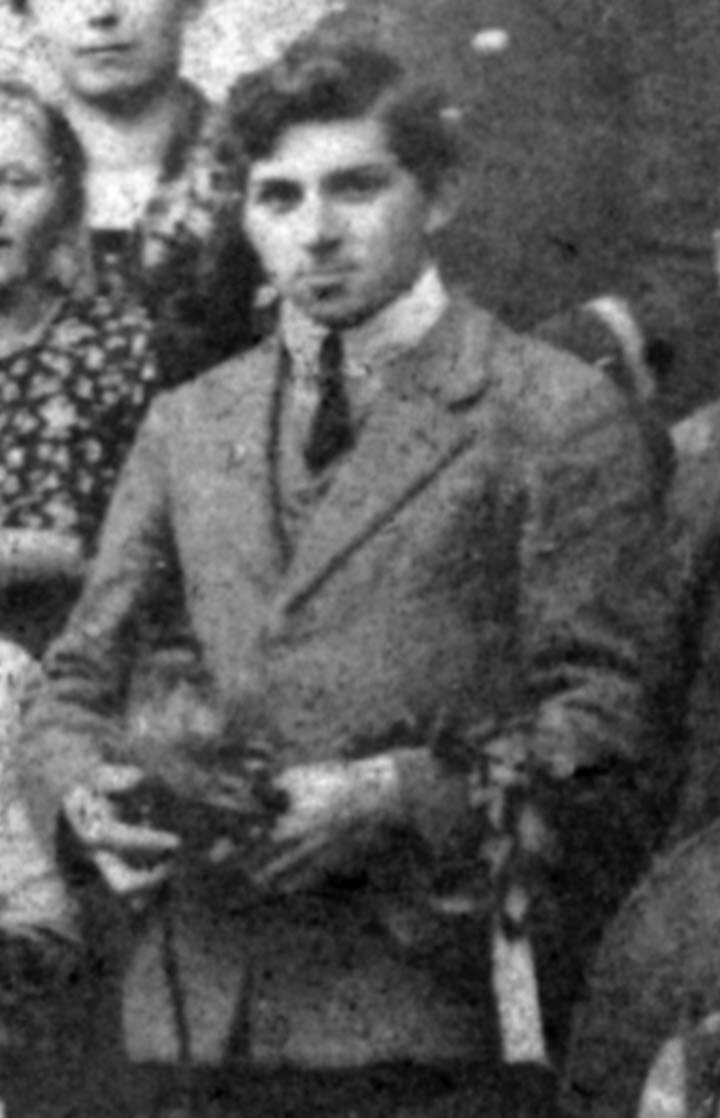
\includegraphics[width=4.209cm,height=6.507cm]{pictures/zulassungsarbeit-img027.jpg}

Abb. \stepcounter{Abb}{\theAbb}: Max Rauscher\\
\end{supertabular}
\end{center}
\end{minipage}
\end{center}
Als Rauscher durch seine Anschuldigung Högn in den Streit mit hineinzog
und dieser mit markigen Worten offen die Kündigung Rauschers verlangte,
wurde eines deutlich: Ihr Verhältnis zueinander war offenbar auch
vorher nicht gut gewesen. Gehörte Högn nicht auch zu den Nörglern, die
schon zu Beginn von Rauschers Dienstzeit wenig Vertrauen in ihn setzten
und Rauscher während seiner 2-jährigen Dienstzeit die Arbeit schwer
machten, bis er es schließlich mit einer utopischen Gehaltforderung
bewusst auf die Kündigung anlegte? Högn wäre mit Sicherheit gerne
weiterhin Chorregent geblieben, wenn man, abgesehen vom finanziellen
Aspekt, die Abwechslung in der Tätigkeit betrachtet, die der
Chorregentendienst bot, sowie die Tatsache, dass Högn diesen Dienst mit
Leib und Seele ausführte. Die Anstellung Rauschers lieferte
letztendlich den Grund dafür, dass Kirchen- und Schuldienst nicht mehr
von einer Person ausgeübt werden durfte.

Eine Eintragung von Högn in einer Dirigierpartitur aus dem Notenbestand
der Ruhmannsfeldener Kirche ist beredtes Zeugnis dieser Rivalität
zwischen Rauscher und Högn. Rauscher hatte einen vermeintlichen
Vorzeichenfehler in der Partitur einer Messe von Vinzenz Goller
korrigiert. In einem rechthaberischen Ton schrieb Högn, der von der
Richtigkeit des gedruckten Notentextes überzeugt war, später den
Kommentar \zitat{„Grober Fehler! Nein! Muss „des“ heißen!“
}(Abb. 26) dazu, anstatt das eingefügte Vorzeichen einfach
auszuradieren, als hätte er der Nachwelt seine Zweifel an Rauschers
Kompetenz durch die Eintragung in die Partitur, die eigentlich nur er
selbst verwendete, mitteilen wollen.

\begin{center}
\begin{minipage}{4.142cm}
\begin{flushleft}
\tablefirsthead{}
\tablehead{}
\tabletail{}
\tablelasttail{}
\begin{supertabular}{m{3.9420002cm}}

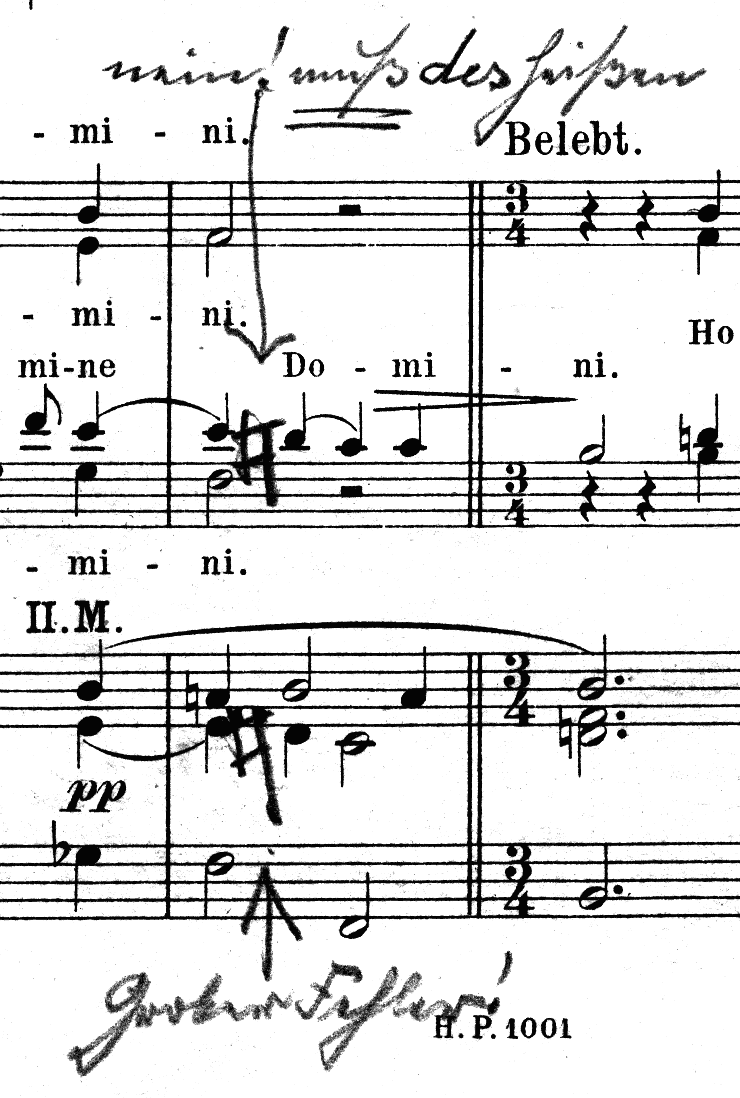
\includegraphics[width=3.759cm,height=5.547cm]{pictures/zulassungsarbeit-img028.png}

\label{bkm:Ref100166968}Abb. \stepcounter{Abb}{\theAbb}: Eintragungen
von Max Rauscher und August Högn in eine Dirigierparitur\\
\end{supertabular}
\end{flushleft}
\end{minipage}
\end{center}
Pfarrer Fahrmeier schrieb nach der Kündigung Rauschers an die Regierung
von Niederbayern einen Brief, der den Zweck erfüllen sollte, eine
Ausnahmegenehmigung für die Übernahme des Chorregentendienstes durch
Högn zu erhalten. Dies zeigt, dass das Verhältnis Fahrmeier und Högn
anscheinend ein sehr gutes war. Nur Högn besitze, diesem Schreiben
zufolge die, \zitat{„zur Übernahme des Kirchenchores
notwendigen musikalischen Fähigkeiten und Kenntnisse“ }\footnote{
Dokument Nr. 12, Brief von der Kirchenverwaltung an die Regierung von
Niederbayern, 1.4.1927} und daher solle die zuständige Behörde den
Chorregentendienst von Högn \zitat{„bis auf weiteres“
} \footnote{Dokument Nr. 12, Brief von der Kirchenverwaltung an die
Regierung von Niederbayern, 1.4.1927} genehmigen. August Högn kannte
Fahrmeier schon lange vor seiner Ruhmannsfeldener Zeit. In Deggendorf
war Fahrmeier als Geistlicher zwischen 1896 und 1918 tätig.\footnote{
Reicheneder-Chronik, Seelsorger, Blatt III/13
(1) Vorderseite} Er konnte als Freund und Hauspfarrer der Familie Högn
in Deggendorf bezeichnet werden. Wenn er zur Ruhmannsfeldener Zeit
einen Ausflug nach Deggendorf unternahm, genehmigte er sich stets im
Hause Högn zuerst ein Bad, bevor er seinen Besorgungen in der Stadt
nachging. \footnote{Interview Nr. 3, Ida Högn, 29.12.2002, Absatz 10}

August Högns zweites Engagement in der Kirche von Ruhmannsfelden sollte
nur von begrenzter Dauer sein. Nur bis zu den Sommerferien 1927 sollte
die Regierung von Niederbayern Högns kirchenmusikalische Tätigkeit
genehmigen, \footnote{Dokument Nr. 13, Brief von der Kirchenverwaltung
an die Regierung von Niederbayern, 22.4.1927} bis ein pensionierter
Lehrer gefunden war, der die Chorregentenstelle längerfristig
übernehmen könnte. Doch unter der Ruhmannsfeldener Bevölkerung erhob
sich heftiger Widerstand gegen die Anstellung eines
Pensionisten, \footnote{Dokument Nr. 14, Brief von Alois Hartl an
Kirchenrat, 15.6.1927; Dokument Nr. 15, Brief von Johann Bielmeier an
Kirchenverwaltung, 17.6.1927} sodass die Stelle öffentlich
ausgeschrieben und von den fünf Kirchenmusiker, \footnote{Dokument Nr.
75, Bewerbung von Gottfried Hagemeiner, 25.10.1927} die sich beworben
hatten, entschied man sich für einen gewissen Georg Roßnagel. Sein
Dienstvertrag wurde zum Unterschreiben für den 7. Juni 1927 aufgesetzt.
Anscheinend hat Roßnagel seinen Dienst nie angetreten, denn derselbe
Dienstvertrag wurde zu einem späteren Zeitpunkt, mit ausgebesserten
Namen noch einmal bei der Anstellung von Albert Schroll verwendet, der
am 31. Juli 1929 diesen Vertrag mit der Kirche in Ruhmannsfelden
abschloss. Während der Name Schroll bei vielen Zeitzeugen bekannt war,
wusste nie etwas von einem Kirchenmusiker mit dem Namen Georg Roßnagel,
der laut Dienstvertrag zwei Jahre lang in Ruhmannsfelden gewirkt haben
soll. \footnote{Dokument Nr. 8, Dienstvertrag für Albert Schroll (Georg
Roßnagel), 31.7.1929 (7.6.1927)} Im Sommer 1929 trat Albert Schroll den
Chorregentendienst in Ruhmannsfelden an. Die auf wenige Wochen
beschränkte Aushilfe durch August Högn hat man am Ende auf über zwei
Jahre verlängert.

\begin{center}
\begin{minipage}{9.638cm}
\begin{center}
\tablefirsthead{}
\tablehead{}
\tabletail{}
\tablelasttail{}
\begin{supertabular}{m{4.333cm}m{4.905cm}}

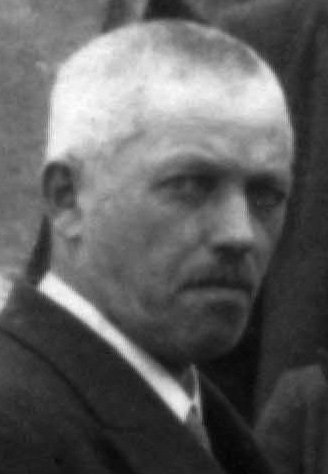
\includegraphics[width=4.15cm,height=6.006cm]{pictures/August-Hoegn_Nachruf.jpg}

Abb. \stepcounter{Abb}{\theAbb}: August Högn &

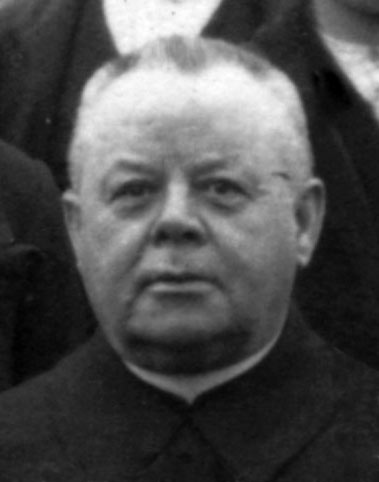
\includegraphics[width=4.722cm,height=5.994cm]{pictures/zulassungsarbeit-img029.jpg}

Abb. \stepcounter{Abb}{\theAbb}: Karl Fahrmeier, in Ruhmannsfelden
Pfarrer von 1918 – 1935\\
\end{supertabular}
\end{center}
\end{minipage}
\end{center}
